\title{Project 3: Collaboration and Competition}
\author{
	Rory McGrath \\
}
\date{\today}

\documentclass[12pt]{article}
\usepackage[margin=1in]{geometry}
\usepackage{graphicx}
\usepackage[backend=bibtex,style=numeric]{biblatex}
\bibliography{References}
\usepackage[table]{xcolor}

\begin{document}
\maketitle


\section{Overview}

In this environment, two agents control rackets to bounce a ball over a net. 
If an agent hits the ball over the net, it receives a reward of +0.1. 
If an agent lets a ball hit the ground or hits the ball out of bounds, it receives a reward of -0.01. 
Thus, the goal of each agent is to keep the ball in play.

The observation space consists of 8 variables corresponding to the position and velocity of the ball and racket. 
Each agent receives its own, local observation. 
Two continuous actions are available, corresponding to movement toward (or away from) the net, and jumping.
The task is episodic, and in order to solve the environment, your agents must get an average score of +0.5 (over 100 consecutive episodes, after taking the maximum over both agents).
Specifically,
\begin{itemize}
\item After each episode, the rewards that each agent received are summed up (without discounting), to get a score for each agent. 
This yields two seperate scores. 
We then take the maximum of these two scores.
\item This yields a single score for each episode.
The environment is considered solved, when the average (over 100 episodes) of those scores is at least +0.5.
\end{itemize}

\section{Methods}
\label{methods}
An Actor-Critic approach was used to solve this problem.
Initially two agents were trained to collaborate together, one agent train on the left side of the net the other trained on the right side.
However, this approach when then replaced by training one agent to play against itself.

In order to train a single agent to play against itself the symmetry of the game was exploited.
The main difference between playing on the left or right side of the court is the sign of the x coordinates in the state space.
To train a single agent all states observations were transformed such that they apperared on the right side of the net.
In order to transform the data the elements in the state vector were multiplied by the following vector:
\begin{equation}
state \circ [-1,1,-1,1,...,-1,1]
\end{equation}
This allowed a single agent that could generalise to both sides of the net to be trained with twice the amount of data.
As the actions are relative to the net the do not have to be transformed.
After the states were transformed the agent was trained using DDPG.

Similar to DQN, DDPG uses deep artifical neural networks as large non-linear function approximators for the value function.
In order to train these function approximators in a stabe and robust way DDPG also uses a Replay Buffer\cite{experience_replay} and updates the target networks with "soft target updates" \cite{ddpg_paper}.
The DDPG maintains four seperate ANNs.
Two are the local and target actor functions and two are the local and target critic functions.
The actor function $\mu(s|\theta^{\mu})$ specifies the current policy by deterministically mapping states to a specific action.
The critic function $Q(s,a)$ is learned using the Bellman equation.
Given that the action space is in the range of -1 to 1 the final activation function in the actor network is a tanh function.
The tanh function is given in equation [\ref{tanh_equation}]
\begin{equation}
\label{tanh_equation}
f(x) = \frac{(e^x - e^{-x})}{(e^x+e^{-x})}
\end{equation}

One issue with learning in continuous space is exploration.
How does the agent explore the environment?
Given that this is an off-policy algorithm we can construct an exploration policy $\mu'$ by adding noise sampled from a noise process $N$.
Adding this noise to the actor policy yields an exploration policy [\ref{exploration_policy}].

\begin{equation}
\label{exploration_policy}
\mu'(s_t) = \mu(s_t|\theta_t^\mu) + N
\end{equation}
When observing the behaviour of the trained agent this exploration can be turned off.

\section{Results}
Using the methodology described above [\ref{methods}] an agent was trained to solve the environment.
The agent was written in pyTorch and was run using the openai gym toolkit.

The ANN used for the actor consisted of an input layer of 24 nodes, one dense hidden layer of 32 nodes and an output layer of 2 nodes.
The activation functions for the input and hidden layer was the rectified linear units (ReLUs). 
The output layers activation function was the hyperbolic tangent function (tanh). 
This maps the output to a range between -1 and 1 which is the required to control moving toward the net and jumping.

The ANN used for the critic has a similar arthecture and consisted of an input layer of 24 nodes, one dense hidden layer of 32 nodes and an output layer of 1 node. 
The action tensor was added to the last hidden layer similar to the paper \cite{ddpg_paper}.

The following hyper-parameters were used to train the agent:

\begin{table}[h!t]
\begin{center}
\begin{tabular}{|c|l|}
	\hline
	\multicolumn{2}{|c|}{\textbf{Learning Updates}}\\
	\hline
	\hline
	\textbf{Parameter} & \textbf{Value}\\
	\hline
	$\gamma$ & $0.99$\\
	$\tau$ & $1e^{-3}$\\
	$\epsilon$ & 1.0 to 0.01 with a rate of decay of 0.995 per episode\\
	\hline
\end{tabular}
\end{center}
\end{table}

\begin{table}
\begin{center}
\begin{minipage}{.3\linewidth}
\begin{tabular}{|c|l|}
	\hline
	\multicolumn{2}{|c|}{\textbf{Experience Replay}}\\
	\hline
	\hline
	\textbf{Parameter} & \textbf{Value}\\
	\hline
	Buffer Size & $1e^{5}$\\
	Batch Size & $1024$\\
	\hline
\end{tabular}
\end{minipage}
\begin{minipage}{.3\linewidth}
\begin{tabular}{|c|l|}
	\hline
	\multicolumn{2}{|c|}{\textbf{Actor Network}}\\
	\hline
	\hline
	\textbf{Parameter} & \textbf{Value}\\
	\hline
		Update Rate & 1 \\
		Learning Rate & $1e^{-4}$ \\
	\hline
\end{tabular}
\end{minipage}
\begin{minipage}{.3\linewidth}
\begin{tabular}{|c|l|}
	\hline
	\multicolumn{2}{|c|}{\textbf{Critic Network}}\\
	\hline
	\hline
	\textbf{Parameter} & \textbf{Value}\\
	\hline
		Update Rate & 1 \\
		Learning Rate & $1e^{-3}$ \\
	\hline
\end{tabular}
\end{minipage}
\end{center}
\end{table}

The model was trained for 1636 episodes. 
After 1,536 episodes the model solved the environment obtaining an average score of over 0.5 for 100 consecitive episodes.
A plot of the reward verses episode number is given in [Fig \ref{results}].

\begin{figure}
	\centering
	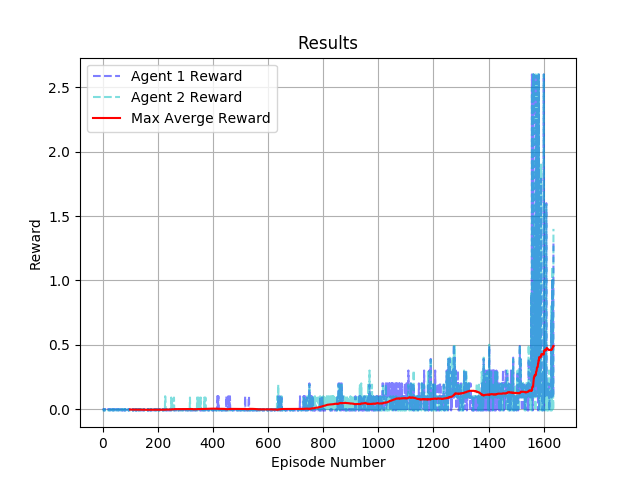
\includegraphics[width=0.8\linewidth]{./img/Results.png}
	\caption{Training results}
	\label{results}
\end{figure}


\section{Future Work}
There are several improvements that could be implemented to decrease training time and increase the average reward.

One of the most difficult aspects of this project was find hyper-aparameter that lead to stable learning.
Trying out variations of hyper-parameters along with different network achitectures was extreamly time consuming.
A hyper-parameter optimisation technique such as grid search could be implemented to help converge on good choices for the parameters 
specified above. 
Here you could set the ranges and combinations you wanted to investigate and run the search on a gpu server.

The Replay Buffer could be updated to implement prioritised experience replay \cite{per_paper}. 
The key idea here is that 'important' transitions would be sampled more frequently than unimportant ones. 
The 'important' of transition is determined by the magnitude of it's temporal-difference error.
This should allow the agent to learn more efficiently. 
Given that we are no longer uniformly sampling from the experiences importance sampling will have to be added to calculate the impact of each weight when updating.

\printbibliography
\end{document}
